\documentclass{standalone}
\usepackage{tikz}
\usetikzlibrary{calc}
\begin{document}
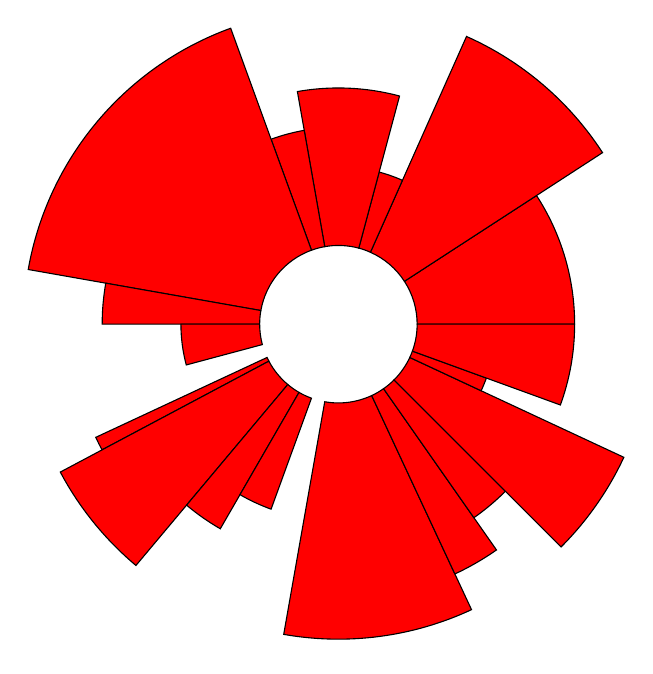
\begin{tikzpicture}
  \coordinate (c) at (0,0);

  \newcommand{\seg}[4]{
    \draw[fill=red]
    ($(c) + (#1:#4)$) arc (#1:#2:#4) --
    ($(c) + (#2:#3)$) arc (#2:#1:#3) -- cycle;
  };

  \seg{0}{33}{1}{3};
  \seg{33}{66}{1}{4};
  \seg{66}{75}{1}{2};
  \seg{75}{100}{1}{3};
  \seg{100}{110}{1}{2.5};
  \seg{110}{170}{1}{4};
  \seg{170}{180}{1}{3};
  \seg{180}{195}{1}{2};
  % Nothing 195-205
  \seg{205}{208}{1}{3.4};
  \seg{208}{230}{1}{4};
  \seg{230}{240}{1}{3};
  \seg{240}{250}{1}{2.5};
  % Nothing 250 260
  \seg{260}{295}{1}{4};
  \seg{295}{305}{1}{3.5};
  \seg{305}{315}{1}{3};
  \seg{315}{335}{1}{4};
  \seg{335}{340}{1}{2};
  \seg{340}{360}{1}{3};

\end{tikzpicture}
\end{document}
